\documentclass[a4paper]{article}
\usepackage[T1]{fontenc}
\usepackage[polish]{babel}
\usepackage[utf8]{inputenc}
\usepackage{lmodern}
\selectlanguage{polish}

\usepackage[margin=1 in, includefoot]{geometry}
\pagenumbering{arabic}
\setcounter{page}{2}
\usepackage{graphicx}
\usepackage{float}
\usepackage{multirow}
\usepackage[space]{grffile}
\usepackage{xcolor, listings}
\usepackage{mathtools}
\lstset{
basicstyle=\footnotesize\ttfamily,
numbers=left,
numberstyle=\tiny,
numbersep=5pt,
tabsize=2,
extendedchars=true,
breaklines=true,
commentstyle=\color{green},
keywordstyle=\color{blue},
identifierstyle=\color{black},
showspaces=false,
showstringspaces=false,
}
\lstdefinestyle{sharpc}{language=[Sharp]C, frame=lr, rulecolor=\color{blue!80!black}}
%nowa strona przed kazdym section
\let\oldsection\section
\renewcommand\section{\clearpage\oldsection}
\newcommand\tab[1][1cm]{\hspace*{#1}}
\begin{document}
\begin{titlepage}
\begin{center}
\huge{\textsc{Politechnika Wrocławska\\Wydział Elektroniki}}
\line(1,0){400}\\
[1 cm]
\textsc{\Huge {Zarządzanie w Systemach i Sieciach Komputerowych}}\\
[0.5 cm]
\textsc{\Large {Optymalizacja listy zakupów pod względem ceny}}\\
\end{center}
\vfill
\vfill
\hspace{0.5 cm}
\begin{minipage}[t]{.4\textwidth}%
\flushleft
\textsc{\Large{Autorzy :}}\\
\Large{Rafał Gubała }\\
\Large{Jakub Małyjasiak}
\end{minipage}%
\begin{minipage}[t]{.5\textwidth}%
\flushright
\textsc{\Large{Prowadzący :}}\\
\Large{dr inż. Robert Wójcik}\\
\end{minipage}%
\vfill
\begin{center}
\normalsize{Wrocław 2017}
\end{center}
\end{titlepage}

\tableofcontents 
\listoffigures

\section{Wstęp}
\subsection{Cel projektu}
\large
Celem projektu było opracowanie i stworzenie aplikacji na platformę Windows implementującą algorytmy optymalizujące listy zakupowe pod względem ceny produktów z różnych sklepów.
\subsection{Zakres projektu}
\large
Założenie projektowe obejmowały stworzenie aplikacji okienkowej posiadającej następujące funkcjonalności:
\begin{itemize}
\item Dodawanie, edycja oraz usuwanie sklepów
\item Dodawanie, edycja oraz usuwanie produktów
\item Tworzenie list zakupowych z wybranymi produktami
\item Optymalizacja list zakupowych algorytmami \textbf{Shop-Enum} oraz \textbf{Product-Enum}
\item Mierzenie czasu wykonywania się poszczególnych algorytmów
\item Zapisywanie i wczytywanie wprowadzonych danych
\end{itemize}
\section{Sformułowanie problemu}
\subsection{Podstawowe założenia}
\large
Rozwiązywany problem dotyczy zakupów internetowych i zminimalizowania kosztów poniesionych przy zakupie wybranych produktów w wybranych sklepach. Pojedyncza osoba szuka określonego zestawu produktów $N = \{1,...,n\}$ w $m$ sklepach. Każdy sklep posiada swój koszt wysyłki $d_i$ oraz każdy podzbiór produktów $N_i$ może być skojarzony z wieloma sklepami. Oprócz tego, każdy produkt należący do wybranego podzbioru $N_i$ posiada swoją cenę $c_{ji}$, gdzie $j \in N_i$ Rozwiązaniem problemu jest znalezienie takiego zestawu produktów z co najmniej jednego sklepu, aby sumaryczna wartość zakupów była jak najmniejsza.
\subsection{Opis wariantów problemu}
\subsubsection{Problem decyzyjny}
W przypadku obu algorytmów problem decyzyjny sprowadza się do pytania, czy istnieje podzbiór produktów $N_i$ i odpowiadający mu zbiór sklepów $M_i$, dla którego sumaryczny koszt zakupu będzie równy $k$. Rozwiązanie owego problemu będzie polegało na przeszukaniu zbioru wszystkich sklepów w poszukiwaniu produktów w podzbioru $N_i$. Jeśli wszystkie produkty udało się znaleźć, to sumując ceny wszystkich przedmiotów z cenami wysyłki w odpowiednich sklepach możemy udzielić odpowiedzi na postawione pytanie.
\subsubsection{Problem optymalizacyjny}
Mając na uwadze sformułowany wcześniej problem decyzyjny możemy prosto sformułować odpowiadający mu problem optymalizacyjny. W tym przypadku brzmi on: \textit{Ile wynosi najniższy koszt zakupu przedmiotów ze zbioru $N_i$ w zadanym zbiorze sklepów.} Warto zauważyć, że problem w istocie nie jest trywialny. Ważną komplikacją jest fakt, że pod uwagę trzeba wziąć koszt wysyłki danego produktu, co sprawia, że proste przeszukanie sklepów w celu znalezienia najtańszych ofert dla danego produktu nie ma sensu. Czasami bardziej opłacalne może okazać się kupienie droższego produktu, jeśli pozwoli to uniknąć poniesienia kosztów wysyłki w innym sklepie. 
\subsection{Zastosowane algorytmy}
Posiłkując się materiałami zawartymi w [3] do rozwiązania problemu wykorzystaliśmy algorytmy \textit{SHOP-ENUM} oraz \textit{PRODUCT-ENUM}. Oba pozwalają znaleźć optymalne rozwiązanie, ale dzieje się to kosztem złożoności obliczeniowej.

Podstawowym założeniem algorytmu \textit{SHOP-ENUM} jest skupienie się na sklepach, zamiast na produktach. Zakładamy tutaj, że analizie poddamy każdy możliwy podzbiór sklepów, co pozwoli w trywialny sposób przeszukać kolekcję w celu znalezienia najtańszej oferty na dany produkt z punktu widzenia pojedynczej iteracji. Jest to możliwe dzięki temu, że koszt wysyłki nie gra tutaj roli. Ze względu na to, że analizie zostanie poddany każdy podzbiór sklepów, czyli każda możliwa kombinacja kosztów wysyłki, możemy w naiwny sposób szukać podzbioru produktów o najniższej cenie. Koszt wysyłki zwiększa ową cenę o odpowiednią wartość i w ten sposób otrzymujemy rezultat działania algorytmu.
\vspace{0.5 cm}
\lstset{style=sharpc}
\begin{lstlisting}
foreach permutation of stores
		foreach product in shoppingList
			cheapestProduct <- stores.findCheapest(product)
			resultList.add(cheapestProduct)
		
		if resultList.Cost < bestSolution.Cost then
			bestSolution <- resultList
\end{lstlisting}
\vspace{0.5 cm}

Algorytm \textit{PRODUCT-ENUM} to przeciwieństwo wspomnianego wcześniej algorytmu \textit{SHOP-ENUM}. Tutaj uwagę skupia się na produktach. Podstawą algorytmu jest założenie, że tym razem zamiast analizować każdy możliwy podzbiór sklepów, stworzymy każdą pożliwą kombinację produktów. Pseudokod trafnie obrazuje ten zamysł:

\vspace{0.5 cm}
\lstset{style=sharpc}
\begin{lstlisting}
Permutate(shoppingList, stores, itemIndex) {
	if itemIndex < shoppingList.Count then
		foreach store in stores 
			product <-  store.findProduct(shoppingList[itemIndex])
			if product.Amount < shoppingList[itemIndex].Amount then continue
			shoppingList[itemIndex].setNewPrice(product.Price)
			shoppingList[itemIndex].setNewStore(product.Store)
		
			Permutate(shoppingList, stores, itemIndex + 1)
	else
		if shoppingList.Cost < bestSolution.Cost then
			bestSolution <- shoppingList
}
\end{lstlisting}
\vspace{0.5 cm}
Widać tutaj jasno, że naszym zamiarem będzie stworzenie każdej możliwej kombinacji produktów, jak już wcześniej wspomniano. W praktyce oznacza to wykorzystanie rekurencji, która pozwoli na każdej pozycji na liście zakupów przeanalizować wariant, w którym produkt bierzemy kolejno z każdego sklepu, w którym jest dostępny
\subsection{Analiza złożoności obliczeniowej algorytmów}
\subsubsection{Algorytm SHOP-ENUM}
Zauważmy, że skoro algorytm bazuje na utworzeniu wszystkich możliwych kombinacji analizowanych sklepów ze zbioru $\{1,...,m\}$, to wszystkich możliwych kombinacji będzie $2^m$. Następnie należy znaleźć najtańszą ofertę na dany produkt, co w przypadku przechowywania sklepów na liście można otrzymać w czasie $O(m)$, jeśli m to ilość przeszukiwanych produktów. Mamy zatem $2^mm$. Operację wyszukiwania należy powtórzyć dla każdego produktu na liście zakupów, której długość możemy oznaczyć jako $n$. Mamy zatem ostatecznie
\begin{equation}
O(nm2^m)
\end{equation}
Dużą poprawę można byłoby osiągnąć, gdyby oferty produktów były przechowywane w kopcu. Wtedy operacja znalezienie najtańczej oferty, zakładając, że będzie to kopiec minimalny względem ceny, udałoby się wykonać w stałym czasie, a złożoność spadłaby do:
\begin{equation}
O(n2^m)
\end{equation}
\subsubsection{Algorytm PRODUCT-ENUM}
Algorytm \textit{PRODUCT-ENUM}, jak już wcześniej stwierdzono, polega na przeanalizowaniu każdego możliwego zbioru produktów. Jeśli oznaczymy ilość produktów na liście jako $n$, czyli produkty stworzą podzbiór $S = \{S_1,...,S_n\}$, a ilość sklepów przez $m$, to zauważymy, że istnieje $m^n$ takich kombinacji. Daje to złożoność równą $O(m^n)$. Na tym etapie, w przeciwieństwie do algorytmu \textit{SHOP-ENUM}, nie mamy jeszcze żadnej informacji o cenie produktów. Jeśli, jak już ustaliliśmy, podzbiór składa się z $n$ elementów, to dodając ten etap do dotychczasowej złożoności otrzymujemy:
\begin{equation}
O(nm^n)
\end{equation}
\section{Projekt aplikacji}
\subsection{Wykorzystywane technologie i narzędzia projektowania}
Do stworzenie projektu zostały użyte następujące technologie i narzędzia:
\begin{itemize}
\item Język programowania: C\#
\item Środowisko programistyczne: Visual Studio 2015, Visual Studio 2017
\item XAML - język opisu interfejsu użytkownika
\item Inne: WPF, NewtonSoft: JSON.Net
\end{itemize}
\subsection{Struktura programu}
W projekcie został zastosowany wzorzec obiektowy. Aplikacja została napisana z rozdzieleniem interfejsu użytkownika oraz logiki samych algorytmów minimalizujących w postaci odrębnych modułów (projektów w solucji). Zabieg ten miał na celu wyodrębnić moduł algorytmiczny, aby można go było łatwo przenieść w przyszłości do innego projektu np. w postaci skompilowanej biblioteki.
\begin{flushleft}
Program zapisuje dane do pliku tekstowego w popularnym formacie JSON. Umożliwia to łatwy odczyt i parsowanie tekstu do obiektów w programie. Jest to symulacja bazy danych. Obsługa danych została zrealizowana jako wzorzec fabryki, każda encja posiada swoją fabrykę z metodami takimi jak: \textit{getAll}, \textit{getByID}, \textit{create}, \textit{update} oraz \textit{delete}.
\end{flushleft}
\subsection{Koncepcja działania algorytmów}
Oba algorytmy, jak już wcześniej wspomniano, zostaną umieszczone w osobnym module, co pozwoli lepiej odseparować logikę od widoku oraz wykorzystać skompilowany kod w innych projektach. Dla uproszczenia zostaną wprowadzone dodatkowe obiekty, które lepiej pasują do realizacji algorytmów. 
\subsubsection{Algorytm SHOP-ENUM}
W przypadku tegoż algorytmu konieczne jest znalezienie sposobu na szybkie i oszczędne generowanie kolejnych podzbiorów analizowanych sklepów. Rozwiążemy to tworząc osobną strukturę – tablicę zmiennych logicznych, lub liczb całkowitych takich, ze $x \in \{0, 1\}$ – która będzie stanowiła swego rodzaju maskę bitową. Załóżmy, że  mamy zbiór $\{a, b, c, d\}$ sklepów, a na danym etapie analizie mają podlegać jedynie sklepy \textit{a} oraz \textit{d}. Wtedy maska będzie miała postać $[1, 0, 0, 1]$. Stosują odpowiednie algorytmy możemy regularnie przesuwać maskę uzyskując wszystkie możliwe kombinacje. Następnie konieczne będzie wyszukanie najtańszej oferty sprzedaży danego produktu w dostępnych w danej iteracji sklepach. Do przechowywania danych wykorzystujemy nieposortowane listy – każdy sklep ma listę dostępnych w nim produktów, więc konieczne będzie przejrzenie kolejno wszystkich elementów listy i znalezienie tego, który zawiera najniższą cenę. Cena ta może zostać odrazu dodana do końcowej sumy, co pozwoli uniknąć kolejnego iterowania po liscie zakupów.
\subsubsection{Algorytm PRODUCT-ENUM}
Ze względu na konieczność wygenerowania każdej możliwej kombinacji produkt – sklep najprostszym wyjściem jest zastosowanie rekurencji. Implementacja będzie musiała umożliwiać "rozgałęzianie" na każdej pozycji listy zakupów dla wszystkich sklepów, w których dany produkt jest dostępny i jeśli zostanie osiągnięty ostatni poziom drzewa, obliczyć ceny i zwrócić najkorzystniejszą. Takie rozwiązanie będzie miało znaczną złożoność pamięciową, ponieważ wskutek rekursji powstanie drzewo o $n$–poziomach, a każdy węzeł będzie miał maksymalnie $m$–rozgałęzień, gdzie $n$ - ilość produktów na liście, a $m$ - ilość sklepów. Daje to $m^n$ węzłów końcowych.
\subsection{Diagram klas}
\begin{figure}[H]
\centering
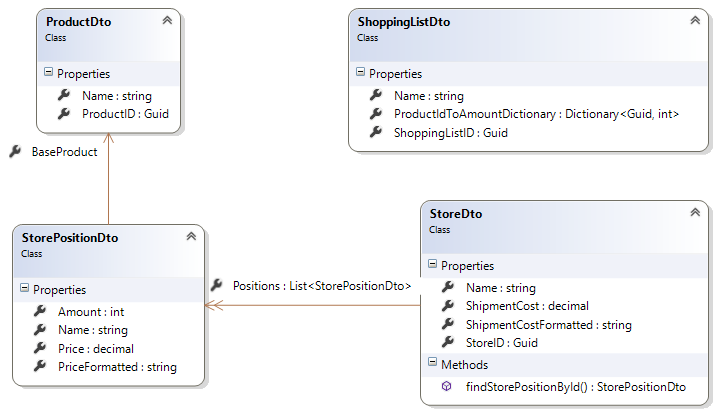
\includegraphics[width=\textwidth,keepaspectratio]{img/diagram-dto.png}
\caption{Diagram klas modeli używanych w module algorytmicznym}
\end{figure}
\begin{figure}[H]
\centering
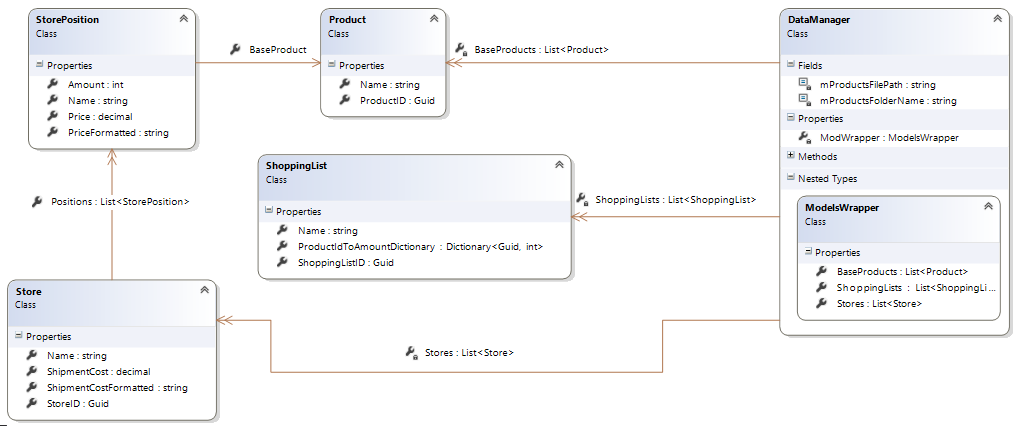
\includegraphics[width=\textwidth,keepaspectratio]{img/diagram-gui.png}
\caption{Diagram klas modeli używanych w interfejsie użytkownika}
\end{figure}
\subsection{Struktura danych wejściowych}
Struktura danych wejściowych algorytmu wygląda następująco:
\begin{itemize}
\item \textit{List<StoreDto> stores} - lista sklepów istniejących w bazie
\item \textit{Dictionary<Guid, int> productsIDToAmount} - słownik przyporządkowujący każdemu wybranemu produktowi (jego identyfikatorowi) z listy zakupowej ilość tego produktu zakupioną przez użytkownika
\item \textit{Algorithm algorithm} - typ wyliczeniowy informujący o tym jaki algorytm będzie zastosowany. Typ \textit{Algorithm} może przyjąć jedną wartość z dwóch do wyboru:
\newline \textit{\textbf{ShopEnum}} lub \textit{\textbf{ProductEnum}}
\end{itemize}
\subsection{Struktura wyników}
Algorytm zwraca obiekt typu \textbf{OptimizedShoppingList}, którego struktura i implementacja wygląda następująco:
\newline
\lstset{style=sharpc}
\begin{lstlisting}
public class OptimizedShoppingList
{
		public List<ShoppingListPosition> Products { get; set; }
    public TimeSpan TimeElapsed { get; set; }
    public decimal TotalPrice { get; set; }

    public OptimizedShoppingList()
    {
    	TotalPrice = decimal.MaxValue;
    }
}
\end{lstlisting}
\newpage
Klasa ta posiada 3 atrybuty:
\begin{itemize}
\item \textit{Products} - lista produktów wytypowanych przez algorytm. Każdy obiekt tej listy posiada informację z jakiego jest sklepu, swój identyfikator, cenę i ilość. Implementacja klasy obiektu z listy:
\newline
\begin{lstlisting}
public class ShoppingListPosition
{
		public StoreDto Store { get; set; }
    public Guid ProductId { get; set; }
    public decimal Price { get; set; }
    public int Amount { get; set; }
}  
\end{lstlisting}
\item \textit{TimeElapsed} - obiekt zawierający informacje o czasie wykonania się algorytmu
\item \textit{TotalPrice} - cena całościowa wytypowana przez algorytm
\end{itemize}
\section{Implementacja systemu}
\subsection{Wybrane klasy}
\subsubsection{ShoppingList}
\lstset{style=sharpc}
\begin{lstlisting}
public class ShoppingList
{
    public Guid ShoppingListID { get; set; }
    public string Name { get; set; }
		public Dictionary<Guid, int> ProductIdToAmountDictionary { get; set; }
}
\end{lstlisting}
\begin{flushleft}
Powyższa klasa reprezentuje listę zakupową. Posiada ona 3 pola: 
\begin{itemize}
\item \textit{ShoppingListID}: identyfikator zrealizowany za pomocą klasy \textbf{Guid} (zapewnia to bardzo dużą losowość)
\item \textit{Name}: nazwa list zakupowej
\item \textit{ProductIdToAmountDictionary}: słownik przyporządkowujący identyfikator produktu na liście do jego ilości
\end{itemize}
\end{flushleft}
\subsubsection{Store}
\lstset{style=sharpc}
\begin{lstlisting}
public class Store
{           
		public Guid StoreID { get; set; }
    public string Name { get; set; }
    public List<StorePosition> Positions { get; set; }
    public decimal ShipmentCost { get; set; }
    public string ShipmentCostFormatted
    {
    		get
        {
        		return this.ShipmentCost.ToString("C");
        }
     }
}
\end{lstlisting}
\begin{flushleft}
Powyższa klasa reprezentuje sklep. Posiada ona 5 pól: 
\begin{itemize}
\item \textit{StoreID}: identyfikator zrealizowany za pomocą klasy \textbf{Guid} 
\item \textit{Name}: nazwa sklepu
\item \textit{Positions}: lista przechowujące pozycje (produkty) sklepowe
\item \textit{ShipmentCost}: cena wysyłki
\item \textit{ShipmentCostFormatted}: sformatowana cena wysyłki, np. "15,00 zł"
\end{itemize}
\end{flushleft}
\subsubsection{Product}
\lstset{style=sharpc}
\begin{lstlisting}
public class Product
{     
	public Guid ProductID { get; set; }      
	public string Name { get; set; }        
}
\end{lstlisting}
\begin{flushleft}
Powyższa klasa reprezentuje produkt. Posiada ona 2 pola: 
\begin{itemize}
\item \textit{ProductID}: identyfikator zrealizowany za pomocą klasy \textbf{Guid} 
\item \textit{Name}: nazwa produktu
\end{itemize}
\end{flushleft}
\subsection{Realizacja algorytmów wyznaczania rozwiązań}
\subsubsection{Algorytm SHOP-ENUM}
Omówienie algorytmu zaczniemy od zaprezentowania kodu, który prezentuje się następująco.
\begin{lstlisting}
using System;
using System.Collections.Generic;
using System.Diagnostics;
using System.Threading;
using KnapsackOptimizer.Model;
using KnapsackOptimizer.Model.Dto;

namespace KnapsackOptimizer.ShopEnum.Logic
{
	public class ShopEnumAlgorithm
	{
		public OptimizedShoppingList Run(Dictionary<Guid, int> shoppingList, List<StoreDto> stores)
		{
			Stopwatch stopwatch = Stopwatch.StartNew();
			var bestShoppingList = new AlgorithmShoppingList(shoppingList);
			bestShoppingList.ComputeCost();
			var currentShoppingList = new AlgorithmShoppingList(shoppingList);

			var subsetMask = new int[stores.Count];
			subsetMask[0] = -1;

			while (GetNextPermutation(subsetMask) != 1)
			{
				for (var i = 0; i < stores.Count; i++)
				{
					if (subsetMask[i] == 0) continue;
					currentShoppingList.Products.ForEach(shopEnumPosition =>
					{
						stores[i].Positions.ForEach(position =>
						{
							if (position.BaseProduct.ProductID != shopEnumPosition.ProductId) return;
							if (position.Price >= shopEnumPosition.Price) return;
							if (position.Amount < shopEnumPosition.Amount) return;
							shopEnumPosition.Store = stores[i];
							shopEnumPosition.ProductId = position.BaseProduct.ProductID;
							shopEnumPosition.Price = position.Price;
						});
					});
				}
				currentShoppingList.ComputeCost();
				if (currentShoppingList.Cost < bestShoppingList.Cost)
				{
					var temp = currentShoppingList;
					currentShoppingList = bestShoppingList;
					bestShoppingList = temp;
				}
				currentShoppingList.Clear();
			}
			stopwatch.Stop();
			var stopwatchElapsed = stopwatch.Elapsed;
			stopwatch = null;
			return bestShoppingList.ToOptimizedShoppingList(stopwatchElapsed);
		}
		
		private int GetNextPermutation(int[] subsetMask)
		{
			int carry = 1;
			int index = 0;
			while (carry == 1 && index < subsetMask.Length)
			{
				subsetMask[index] += 1;
				carry = subsetMask[index] / 2;
				subsetMask[index] %= 2;
				index++;
			}

			return carry;
		}
	}
}
\end{lstlisting}
Jak widać, algorytm został podzielony na dwie części. Jedna, będąca szkieletem, odpowiada za obliczanie kolejnych kosztów i kompletowanie listy zakupów, a druga generuje kolejne kombinacje sklepów, które podlegają dalszej analzie, czyli wśród których szukamy produktów do skompletownia listy zakupów. 

Pierwsza, czyli szkielet, odpowiada sa utworzenie listy zakupów, dla każdej wygenerowanej kombinacji sklepów, co zostało już wspomniane. Algorytm kończy działanie w momencie, kiedy wszystkie kombinacje zostały przejrzane. Zwraca wtedy najkozystniejszą opcję, która jest przechowywana w zmiennej \textit{bestShoppingList}. Wewnątrz, każdy sklep, który jest analizowany w danej kombinacji, jest przeszukiwany w celu znalezienia ofert na dany przedmiot. Jeśli óW przedmiot znajduje się w sklepie, to jest sprawdzana jego cena i w przypadku, jeśli jest ona bardziej krozystna, niż do tej pory znaleziona, sklep zostaje powiązany z danym produktem. Po zakończeniu analizy danej kombinacji następuje obliczenie kosztu dla danej listy zakupów i jeśli udało się znaleźć wszystkie przedmioty oraz nowa cena jest niższa od dotychczasowego najlpszego rozwiązania, to aktualna lista i najlepsza zostają zamienione miejscami. Zamiana nie jest w tym przypadku niezbędna, ale pozwala uniknąć konieczności kolejnej alokacji pamięci. Wykorzystujemy dotychczas zaalokowaną strukturę.

\subsubsection{Algorytm PRODUCT-ENUM}
Opis realizacji modułu zaczniemy od zaprezentowania kodu. Wygląda on następująco.
\begin{lstlisting}
using System;
using System.Collections.Generic;
using System.Diagnostics;
using KnapsackOptimizer.Model;
using KnapsackOptimizer.Model.Dto;

namespace KnapsackOptimizer.ProductEnum.Logic
{
	public class ProductEnumAlgorithm
	{
		private AlgorithmShoppingList BestSolution;
		public OptimizedShoppingList Run(Dictionary<Guid, int> shoppingList, List<StoreDto> stores)
		{
			Stopwatch stopwatch = Stopwatch.StartNew();
			BestSolution = new AlgorithmShoppingList(shoppingList);    
			var shopEnumProducts = new AlgorithmShoppingList(shoppingList);
			Permutate(shopEnumProducts, stores, 0);
			stopwatch.Stop();
			return BestSolution.ToOptimizedShoppingList(stopwatch.Elapsed);
		}

		private void Permutate(AlgorithmShoppingList list, List<StoreDto> stores, int itemIndex)
		{
			if (itemIndex < list.Products.Count)
			{
				foreach (var store in stores)
				{
					var storePosition = store.findStorePositionById(list.Products[itemIndex].ProductId);
					if (storePosition.Amount < list.Products[itemIndex].Amount) continue;
					list.Products[itemIndex].Price = storePosition.Price;
					list.Products[itemIndex].Store = store;

					Permutate(list, stores, itemIndex + 1);
				}
			}
			else
			{
				list.ComputeCost();
				if (list.Cost >= BestSolution.Cost) return;
				BestSolution.Products = list.Products;
				BestSolution.Cost = list.Cost;
			}
		}
	}
}

\end{lstlisting}

Tym razem również algorytm został podzielony na dwie części, ale w przeciwieństwie do algorytm \textit{SHOP-ENUM}, główna funkcjonalność nie znajduje się w szkieletowej funkcji. Tym razem znacznie wygodniej było oprzeć się na rekurencji. W tym celu powstała wywoływana rekurencyjnie funkcja \textit{Permutate}. Rozwiązuje to problem wygenerowania wszystkich możliwych powiązań sklep-produkt. Innymi słowy, chcemy znaleźć wszystkie możliwe sposoby na zrealizowanie listy zakupów.

Funkcja \textit{Permutate} dostaje argumenty \textit{list, stores} oraz \textit{itemIndex}. \textit{List} to po prostu lista zakupów, na której zapisywane są powiązania produkt-sklep. \textit{Stores} to lista dostępnych sklepów, natomiast \textit{item index} odpowiada na pozycję na której funkcja ma dokonać rozgałęzienia. W praktyce polega to na tym, że dla każdej kolejnej pozycji na liście zakupów dokonujemy rozgałęzienia, z których każde odpowiada jednemy ze sklepów, w którym można dany produkt kupić. Funkcja końcy rozgałęzianie, jeśli \textit{item index} jest równy ilości przedmiotów na liście. Wtedy dla każdego rozgałęzienia, których jest $m^n$, obliczana jest cena, którą następnie porównujemy do najlepszej znalezionej.
\newpage
\subsection{Metoda odczytu danych wejściowych}
Dane wejściowe jak zostało to wspomniane wcześniej zapisywane są w formacie \textbf{JSON} do pliku tekstowego. Przykładowy fragment:
\begin{figure}[H]
\centering
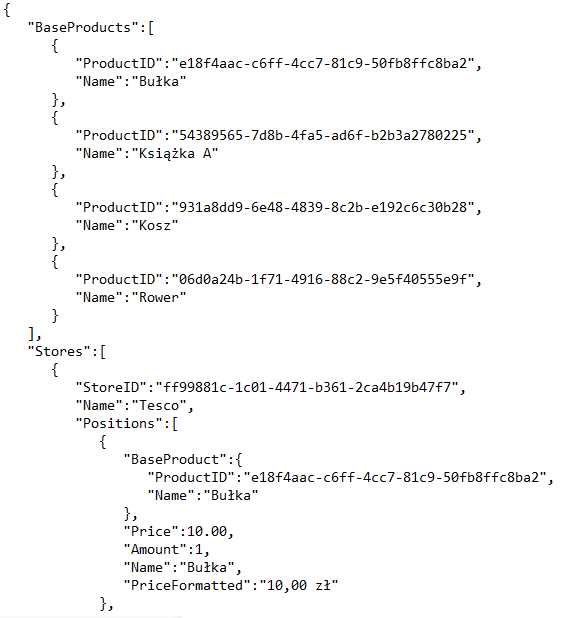
\includegraphics[width=\textwidth,keepaspectratio]{img/json.png}
\end{figure}
\newpage
Do odczytywania danych użyta została biblioteka \textbf{Json.NET - NewtonSoft}. W celu odczytania danych należało posłużyć się instrukcją:
\begin{lstlisting}
this.ModWrapper = JsonConvert.DeserializeObject<ModelsWrapper>(strJson)
\end{lstlisting} 
\begin{flushleft}
Obiekt \textit{ModWrapper} jest obiektem przechowującym dane przy zapisie lub odczycie. Przy odczycie biblioteka pobiera cały plik i deserializuje zapisanego tam JSON-a do obiektu. Struktura i implementacja obiektu \textit{ModWrapper} wygląda następująco:
\end{flushleft}
\begin{lstlisting}
private class ModelsWrapper
{
		public List<Product> BaseProducts { get; set; }
    public List<Store> Stores { get; set; }
    public List<ShoppingList> ShoppingLists { get; set; }
}
\end{lstlisting}
Klasa zawiera 3 atrybuty:
\begin{itemize}
\item \textit{BaseProducts} - lista produktów (sam wzorzec produktu)
\item \textit{Stores} - lista sklepów
\item \textit{ShoppingLists} - lista z obiektami reprezentującymi listy zakupowe
\end{itemize}
\subsection{Metoda prezentacji i zapisu wyników}
Dane prezentowane są zarówno w oknie głównym aplikacji jak i w pojedynczych mniejszych okienkach (popupach). Oto kilka przykładów:
\newline
\begin{figure}[H]
\centering
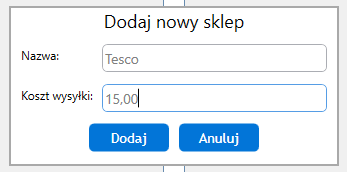
\includegraphics[width=\textwidth,keepaspectratio]{img/modal-nowy-sklep.png}
\caption{Dodawanie nowego sklepu}
\end{figure}
\begin{flushleft}
W tym oknie użytkownik może zdefiniować nowy sklep. Informacje, które należy podać to nazwa sklepu oraz koszt wysyłki produktów.
\end{flushleft}
\begin{figure}[H]
\centering
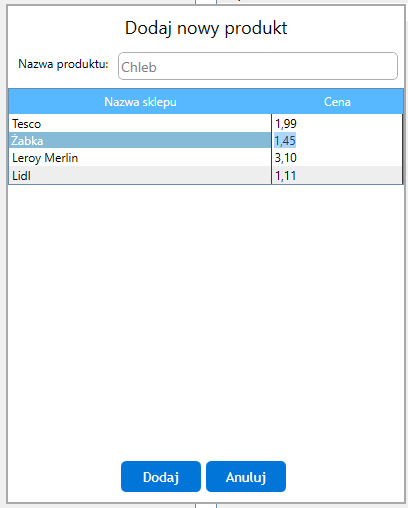
\includegraphics[width=\textwidth,keepaspectratio]{img/modal-nowy-produkt.png}
\caption{Dodawanie nowego produktu}
\end{figure}
\begin{flushleft}
W tym oknie użytkownik dodaje nowy produkt. Może wpisać jego nazwę oraz ile dany produkt kosztuje w każdym ze zdefiniowanych wcześniej sklepów.
\end{flushleft}
\begin{figure}[H]
\centering
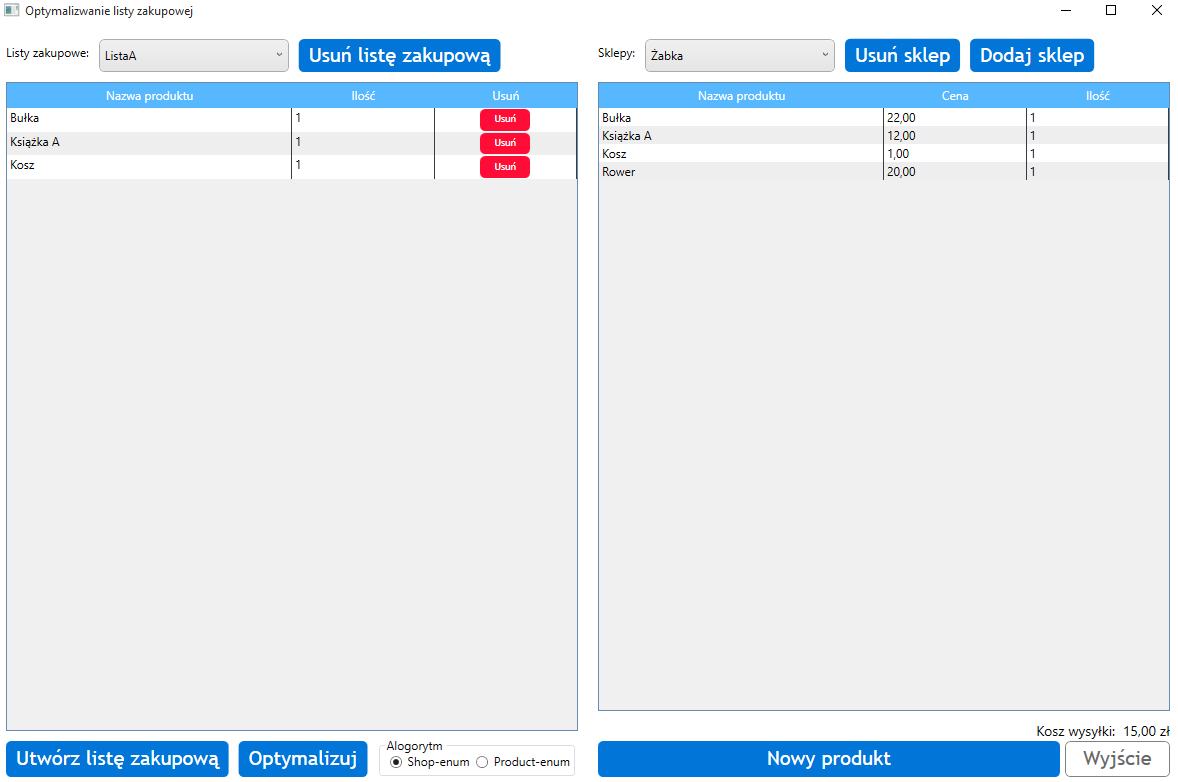
\includegraphics[width=\textwidth,keepaspectratio]{img/main.png}
\caption{Główne okno aplikacji z edycją list zakupowych oraz pozycji sklepowych}
\end{figure}
\begin{flushleft}
W głównym oknie aplikacji użytkownik może zarządzać listami zakupowymi, może je usuwać, zmieniać na nich produkty oraz usuwać produkty z listy. Listy zakupowe wybiera się z listy rozwijanej w lewym górnym rogu. W tym oknie można również zarządzać sklepami. Sklepy wybiera się z listy rozwijanej obok przycisku z napisem "Usuń sklep".
\end{flushleft}
\begin{figure}[H]
\centering
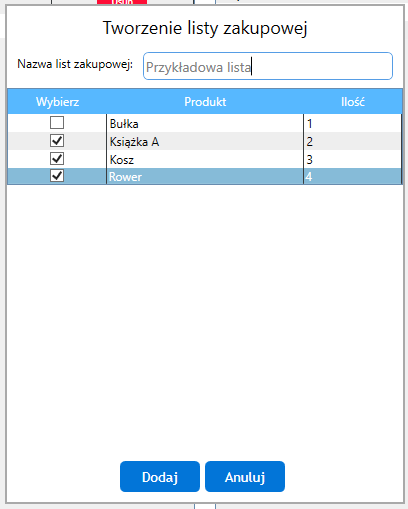
\includegraphics[width=\textwidth,keepaspectratio]{img/modal-nowa-lista.png}
\caption{Tworzenie listy zakupowej}
\end{figure}
\begin{flushleft}
W tym oknie użytkownik może wybrać, które istniejące produkty chce dodać do nowej listy zakupowej wraz z pożądaną ilością oraz może wpisać nazwę tej listy.
\end{flushleft}
\begin{figure}[H]
\centering
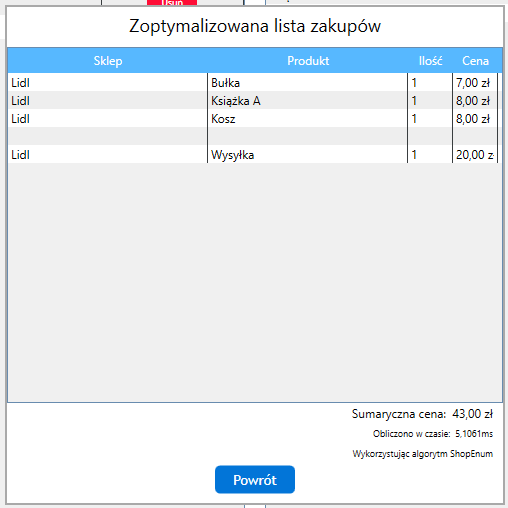
\includegraphics[width=\textwidth,keepaspectratio]{img/modal-optymalizacja.png}
\caption{Prezentacja wyniku algorytmu}
\end{figure}
\begin{flushleft}
Okno z wynikiem algorytmu prezentuje produkty, które zostały dodane do listy. Każdy produkt posiada informację z którego sklepu powinien być kupiony w celu optymalizacji kosztów. Okno to prezentuje również cenę sumaryczną za zakupy, czas poświęcony na optymalizację oraz informację jaki algorytm był użyty.
\end{flushleft}
\section{Testowanie poprawności i ocena rozwiązań}
\subsection{Testy jednostkowe}
\subsection{Weryfikacja poprawności działania algorytmów - przykłady}
\subsubsection{Algorytm SHOP-ENUM}
\subsubsection{Algorytm PRODUCT-ENUM}
\subsection{Analiza czasów wykonania algorytmów}
\subsection{Wnioski z testów i badań}

\section{Podsumowanie}
Reasumując, wykonując ten projekt nauczyliśmy się wielu rzeczy. Przede wszystkim poznaliśmy ciekawe i praktyczne algorytmy do rozwiązywanego przez nas problemu, a także rozwinęliśmy swoją wiedzę na temat .NET oraz tworzenia aplikacji okienkowych z użyciem technologii XAML. Ważnym elementem naszej pracy była również zdolność komunikacji oraz pójścia na kompromis w niektórych sytuacjach. Ważna okazała się również synchronizacja pracy i planowanie kolejnych zadań w taki sposób, aby nie przeszkadzać sobie nawzajem.
\begin{thebibliography}{9}

\bibitem{greene}
  Greene Jennifer, Stellman Andrew 
  \emph{C\#. Rusz głową!}.
  Helion,
  2014.
  
\bibitem{wpf}
	Nathan Adam
	\emph{WPF 4.5 Księga eksperta}. Helion, 2015.  
  
\bibitem{article_algorithms}
	Jacek Błażewicz, Mikhail Y. Kovalyov, Jędrzej Musiał, Andrzej P. Urbanski, Adam Wojciechowski
	\emph{Internet shopping optimization problem}.
	Int. J. Appl. Math. Comput. Sci., 2010, Vol. 20, No. 2, 385–390 
	
  \end{thebibliography}
\end{document}
